\subsection{Current two-arm precursor result and what it does not establish}

The earlier matched experience benchmark supplies a useful precursor measurement for this paper's four-arm attribution programme. After two preserved response-interface failures, the frozen v1.2 RESET-versus-LEARNING packet completed native job 3476548 with twelve of twelve schema-valid records and the intended chronology: RESET tasks begin from the registered initial state; LEARNING development forms a single $S_0\rightarrow S_n$ chain; and every fresh-transfer LEARNING task starts independently from the same frozen $S_n$.

On the staged Qwen2.5-0.5B-Instruct model, both arms achieved zero registered successes on both development and fresh-transfer tasks. The development score delta is zero, and the small partial-score difference on fresh transfer does not satisfy the registered success criterion or grant a global capability claim. The bound result is therefore a scoped negative:
\path{NEGATIVE_NO_TRANSFER_SUCCESS_LIFT_UNDER_0_5B}.
The earlier v1 and v1.1 executions remain in the lineage as prompt-interface failures rather than being pooled with the interpretable v1.2 result.

This measurement matters for Method-Evolution Mechanics for two reasons. First, it demonstrates that a frozen longitudinal state chronology can survive a real model execution while preserving null and interface-failure outcomes. Second, the zero-success ceiling shows why repository growth, learned-state existence or a small partial-score delta cannot be used as evidence that the method improved. A weak base model can place both RESET and LEARNING below the task's valid-success threshold, making a causal learning effect scientifically unidentifiable at that operating point.

A subsequent Phase-1 ORACLE upper-bound at 0.5B (v1.3 jobs 3476730/3476731) is parse-valid at success rate $0/3$ and classifies \path{MODEL_CAPABILITY_FLOOR_0_5B}. That floor is reported as a model/task operating-point constraint; it does not authorize a capability staircase or promotional lift from the precursor.

The result does not substitute for the four-arm study. It contains no \texttt{MODEL\_ONLY} or \texttt{RAKL\_SHAM\_MEMORY} arm, does not estimate static architecture lift or memory-content-specific lift, and uses one small model and six registered tasks. The paper therefore treats job 3476548 as a scoped negative precursor that constrains model/task selection and confirms the reporting discipline; four-arm confirmatory execution, CONTENT-specific memory lift and model-level learning-efficacy claims remain \textbf{unlicensed} while \path{CAPABLE_MODEL_AVAILABLE}=\path{NO_REFUTED}.

A subsequent 1.5B ORACLE overlay (v1.3\_1) first records job 3476742 as preserved \path{INSTRUMENT_DEFECT} negative history (success $0/3$, parse-valid $1/3$). After the PR~\#343 harness repair, re-run job 3476756 is parse-valid $3/3$ at success rate $0/3$ and classifies \path{MODEL_CAPABILITY_FLOOR_1_5B}; it does not authorize a staircase or license promotional lift.

Further ORACLE overlays at 3B (v1.3\_2 job 3476778; \path{MODEL_CAPABILITY_FLOOR_3B}) and 7B (v1.3\_3 job 3476788; \path{MODEL_CAPABILITY_FLOOR_7B}, success $1/3$, parse-valid $3/3$) exhaust the preregistered capability ladder. A sealed-task V2\_0\_EXEC revisit at 7B (job 3476813) is parse-valid $5/5$ at success rate $2/5$ and classifies \path{MODEL_CAPABILITY_FLOOR_7B_V2_EXEC}. \path{CAPABLE_MODEL_AVAILABLE} remains \path{NO_REFUTED}; the four-arm confirmatory execution therefore stays unauthorized until a newly preregistered capability protocol clears. The failed ladder is not extended post hoc by shopping larger models. Figure~\ref{fig:capability-ladder} shows the full ladder against the registered pass gate.

This capability-limited causal terminal is independent of the structured routing result in Section~\ref{sec:ot-memory}. The latter tests whether already-structured method state is governed correctly; it does not use the failed capability ladder as evidence that an LLM can infer or exploit that state from raw research tasks.

\begin{figure}[t]
\centering
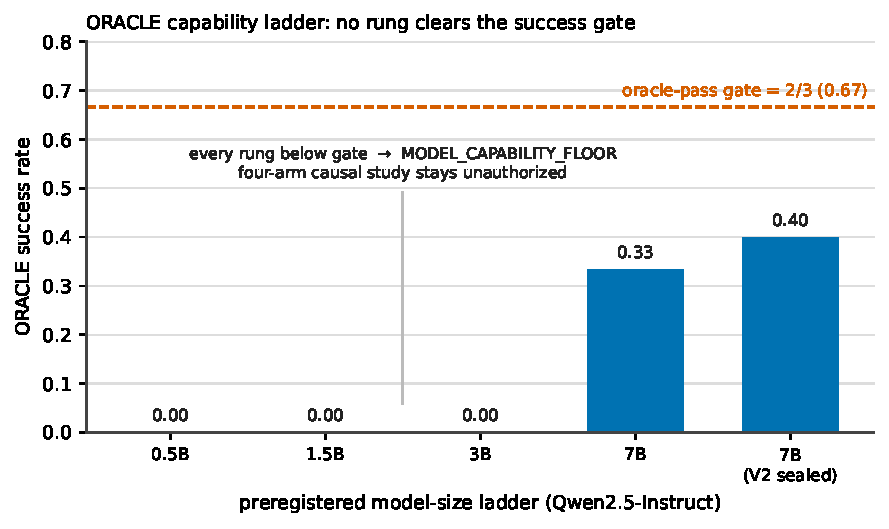
\includegraphics[width=0.68\textwidth]{figures/capability_ladder.pdf}
\caption{Preregistered ORACLE capability ladder for the ExperienceBenchmark upper-bound arm. Success rate rises with model size ($0/3$ at 0.5B, 1.5B and 3B; $1/3$ at 7B; $2/5$ on the sealed V2 revisit at 7B) but no rung reaches the registered oracle-pass gate of $2/3$ (dashed). Every rung is therefore classified \texttt{MODEL\_CAPABILITY\_FLOOR}, leaving \texttt{CAPABLE\_MODEL\_AVAILABLE}=\texttt{NO\_REFUTED}. At a floor the RESET and LEARNING arms are unidentifiable, so the precursor null cannot be read as evidence for or against method learning.}
\label{fig:capability-ladder}
\end{figure}
